\textbf{Входные параметры:} 
 
x --- входная переменная;
 
X --- выборка: значения входов;
 
Y --- выборка: соответствующие значения выходов;
 
VMHL\_N --- размер выборки;
 
C --- коэффициент размытости;
 
V --- тип ядра
 
 \begin{itemize}
 \item  0 --- прямоугольное (не рекомендуется);
 \item  1 --- треугольное;
 \item  2 --- параболическое (считается оптимальным);
 \item  3 --- экспоненциальное;
 \end{itemize}
 
b --- сюда возвращается 1, если все прошло хорошо и 0, если C не захватывает никаких точек выборки (тогда функция возвращает 0).

\textbf{Возвращаемое значение:}
 
 Восстановленное значение производной функции в точке.

\textbf{Формула:}
\begin{eqnarray*}
{f}'\left( x, \overline{X},\overline{Y}, c\right) =\dfrac{\sum_{i=1}^{N}\overline{Y}_i{\Phi}'\left( \frac{x-\overline{X}_i}{c}\right) \sum_{i=1}^{N}\Phi\left( \frac{x-\overline{X}_i}{c}\right)-\sum_{i=1}^{N}{\Phi}'\left( \frac{x-\overline{X}_i}{c}\right) \sum_{i=1}^{N}\overline{Y}_i\Phi\left( \frac{x-\overline{X}_i}{c}\right)}{c\left( \sum_{i=1}^{N}\Phi\left( \frac{x-\overline{X}_i}{c}\right)\right)^2 }.
\end{eqnarray*}

 \begin{figure} [h] 
   \center
   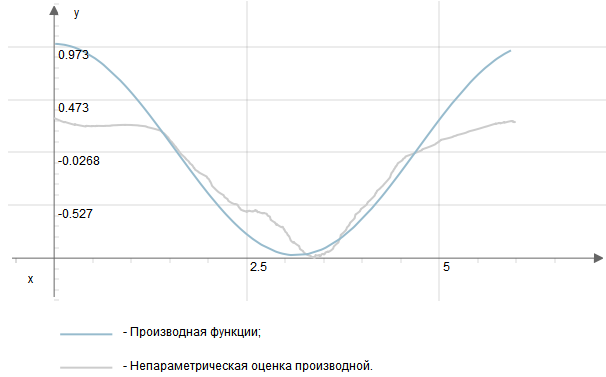
\includegraphics {MHL_NonparametricEstimatorOfDerivative.png}
   \caption{Пример работы функции} 
   \label{img:MHL_NonparametricEstimatorOfDerivative}  
 \end{figure}